\documentclass{article}
\usepackage[utf8]{inputenc}
\usepackage{setspace}
\usepackage{graphicx}
\usepackage{titling}
\usepackage{textcomp}
\usepackage[nottoc]{tocbibind}
\usepackage{tocloft}
\usepackage{natbib}
\usepackage{amsmath}
\usepackage{amssymb}
\usepackage{subcaption}
\usepackage{fontspec}
\renewcommand{\cftsecleader}{\cftdotfill{\cftdotsep}}

\usepackage[margin=1.5in]{geometry}
\addtolength{\topmargin}{-0.5in}
\addtolength{\textheight}{1.0in}

\doublespacing
\newenvironment{bottompar}{\par\vspace*{\fill}}{}

\renewcommand{\contentsname}{\center{Table of Contents}}

\title{Real-time Video Alignment and Fusion Using Feature Detection on FPGA Devices}

\author{Robert Haywood Taglang}

\begin{document}
\pagenumbering{gobble}
\begin{titlingpage}
    \vspace*{\fill}
    \begin{center}
        \textbf{\thetitle}
        
        \hfill \\
        \hfill \\
        
        A Thesis \\
        Submitted to the Faculty \\
        of \\
        Drexel University \\
        by \\
        \theauthor \\
        in partial fulfillment of the \\
        requirements for the degree \\
        of \\
        Master of Science in Computer Engineering \\
        June 2017 \\
    \end{center}
    
    \vspace*{\fill}
    
    \begin{figure*}[!b]
    	\centering
       	
\includegraphics[width=0.35\textwidth]{drexel-vert-blue}
    \end{figure*}
\end{titlingpage}

\begin{center}
	\vspace*{\fill}
	
	\textcopyright\  Copyright 2017
	
	Robert H. Taglang. All Rights Reserved.
	
	\vspace*{\fill}
\end{center}
\clearpage

\pagenumbering{roman}
\setcounter{page}{2}
\begin{center}
    \tableofcontents
    \clearpage
    
    \listoftables
    \clearpage
    
    \listoffigures
\end{center}
\clearpage

\hfill \\
\hfill \\
\hfill \\
\hfill \\

\addcontentsline{toc}{section}{Abstract}

\begin{abstract}
    \singlespacing
    \centering
    \thetitle \\
    \theauthor \\
    Prawat Nagvajara, Ph.D. \\
    
    \hfill \\
    \hfill \\
    \hfill \\
    
    \doublespacing
    Video fusion functions as a way to combine the important or useful parts of two or more sequences of images. The scenario presented is the use of Laplacian fusion to produce a single video composed of the fields of view of two cameras whose areas of focus differ substantially. This is not a useful real-time strategy unless the frames can be aligned. This thesis presents a system for detecting features using an FPGA implementation of SURF (Speeded-Up Robust Features), and aligning video streams by applying a transform generated from the key features. 
\end{abstract}

\clearpage

\pagenumbering{arabic}

\section{Background}

\subsection{Introduction}

The fusion of data from two or more sensors has been well-researched \cite{wang_multi-focus_2011} \cite{li_multi-sensor_1994}, though these approaches typically discuss the process of fusing images which have been pre-aligned. Pre-computed transforms used to align the frames of two cameras are not robust to variations. Some approaches have made use of additional hardware sensors in order to correct against these variations \cite{chappell_exploiting_2006}. The approach presented in this thesis seeks to perform this correction completely in hardware using feature detection on a FPGA.

In order to align two images, one is treated as the reference image, and the other is the transform image which needs to be transformed to be aligned with the reference image. As such the problem can be broken into four major components. 

\begin{enumerate}
	\item Detecting feature points in the two images
	\item Computing the transform which maps the transform image into the space of the reference image
	\item Applying the computed transform to the transform image
	\item Fusion of the reference and transformed image
\end{enumerate}

Feature points are detected using some of the techniques from SURF which makes use of Hessian determinants to detect points of interest in multiple scale spaces. High magnitude features are stored in a buffer to be used for computing the transform.

Once the feature points for the two images have been computed and stored in the buffer, the points from the transform image are mapped to their closest point in terms of euclidean distance from the reference set. An orthogonal projection from the transform points to the reference points is created with the transform as the unknown. Singular value decomposition is used to compute the pseudo-inverse of the matrix containing the reference points so it can be premultiplied by the matrix containing the transform points. The result of this product is the transform matrix which maps transform points to reference points with the error minimized in a least-squares sense. This process may need to be repeated multiple times to converge to a local error minimum, a process referred to as iterative closest point.

As the image data streams into hardware, the data is buffered into memory. With the transform computed, the desired address for the output image is decomposed into $x$ and $y$ coordinates, which are transformed and then reformed back into an address which is used to select pixels from the data in memory. In this way, the transform is applied to align the transform image with the reference image.

Finally, the technique of Laplacian fusion is used to combine the aligned images. It effectively selects the highest frequency components from the two images in order to create an output image where the sharpest, focused parts of the two images are combined into one image.

This process is applied continuously in real time. As the data from the camera data streams in, it produces a single fused output image for display with minimal latency. The design choice to use a FPGA rather than a GPU or some other software based approach was made due to the advantages gained from operating with embedded hardware, namely higher portability and lower overall power consumption. 

\subsection{Laplacian Fusion}

Laplacian pyramids of images have their origin as a strategy for image encoding \cite{burt_laplacian_1983}. A gaussian blur is applied to the image, and the image is downsampled to half of its original size. In this context, Gaussian blur refers to applying kernel convolution to this image with a Gaussian kernel. Likewise, a box blur is the application of a uniformly valued, normalized kernel through kernel convolution. Downsampling refers the process of halving the resolution of the image by combining adjacent pixels. Upsampling is the process of doubling the resolution of the image and interpolating the missing values in the new image. The process of blurring and downsampling can be repeated on the resulting image to create a sequence of images representing the original in different scale spaces. This sequence of blurred and downsampled images is known as a Gaussian pyramid. An illustration of a Guassian pyramid for an example image can be seen in Figure \ref{fig_pepper_gaussian_pyramid}.

\begin{figure}[h]
	\centering
	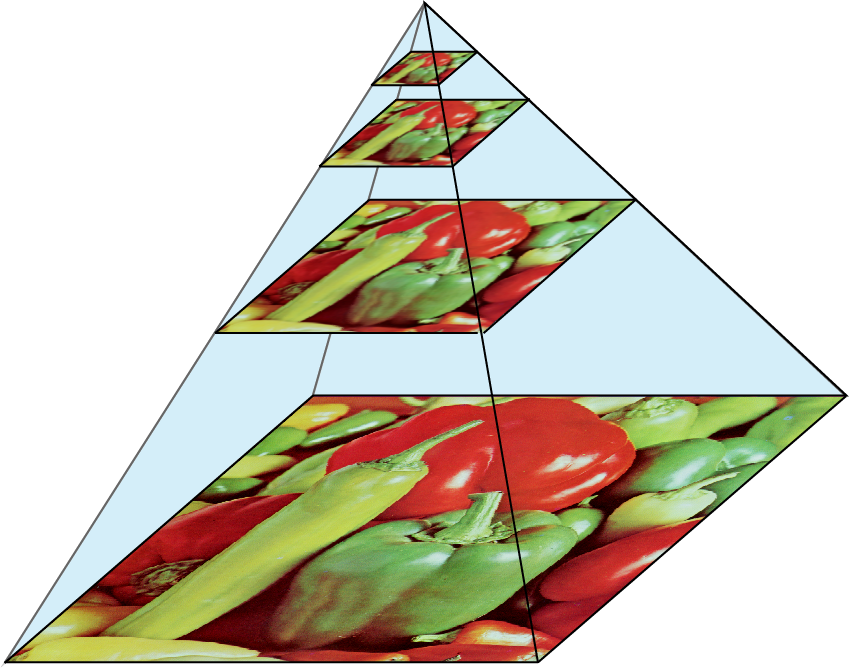
\includegraphics[width=0.6\textwidth]{figures/peppers/gaussian_pyramid}
	\caption{Gaussian pyramid of an example image}
	\label{fig_pepper_gaussian_pyramid}
\end{figure}

The Laplacian pyramid is one which can be used for reconstruction of the original image. At each level above the lowest level of the Gaussian pyramid, the level below is upsampled to match the scale of the current level. The difference between the upsampled image and the current scale level image is known as the Laplacian of the image. The sum of the upsampled lower level and the Laplacian is the original image. At a single level, the Laplacian can be thought of as the error introduced by applying a Gaussian and Box filter. A diagram illustrating a Laplacian pyramid can be seen in Figure \ref{fig_pepper_laplacian_pyramid}. In Figure \ref{fig_pepper_laplacian_pyramid}, the $G\downarrow$ operator refers to applying the Gaussian blur and downsampling, the $\uparrow$ operator refers to upsampling the input image, and the $-$ operator refers to computing the difference of the two input 
images on each channel.
\begin{figure}[h]
	\centering
	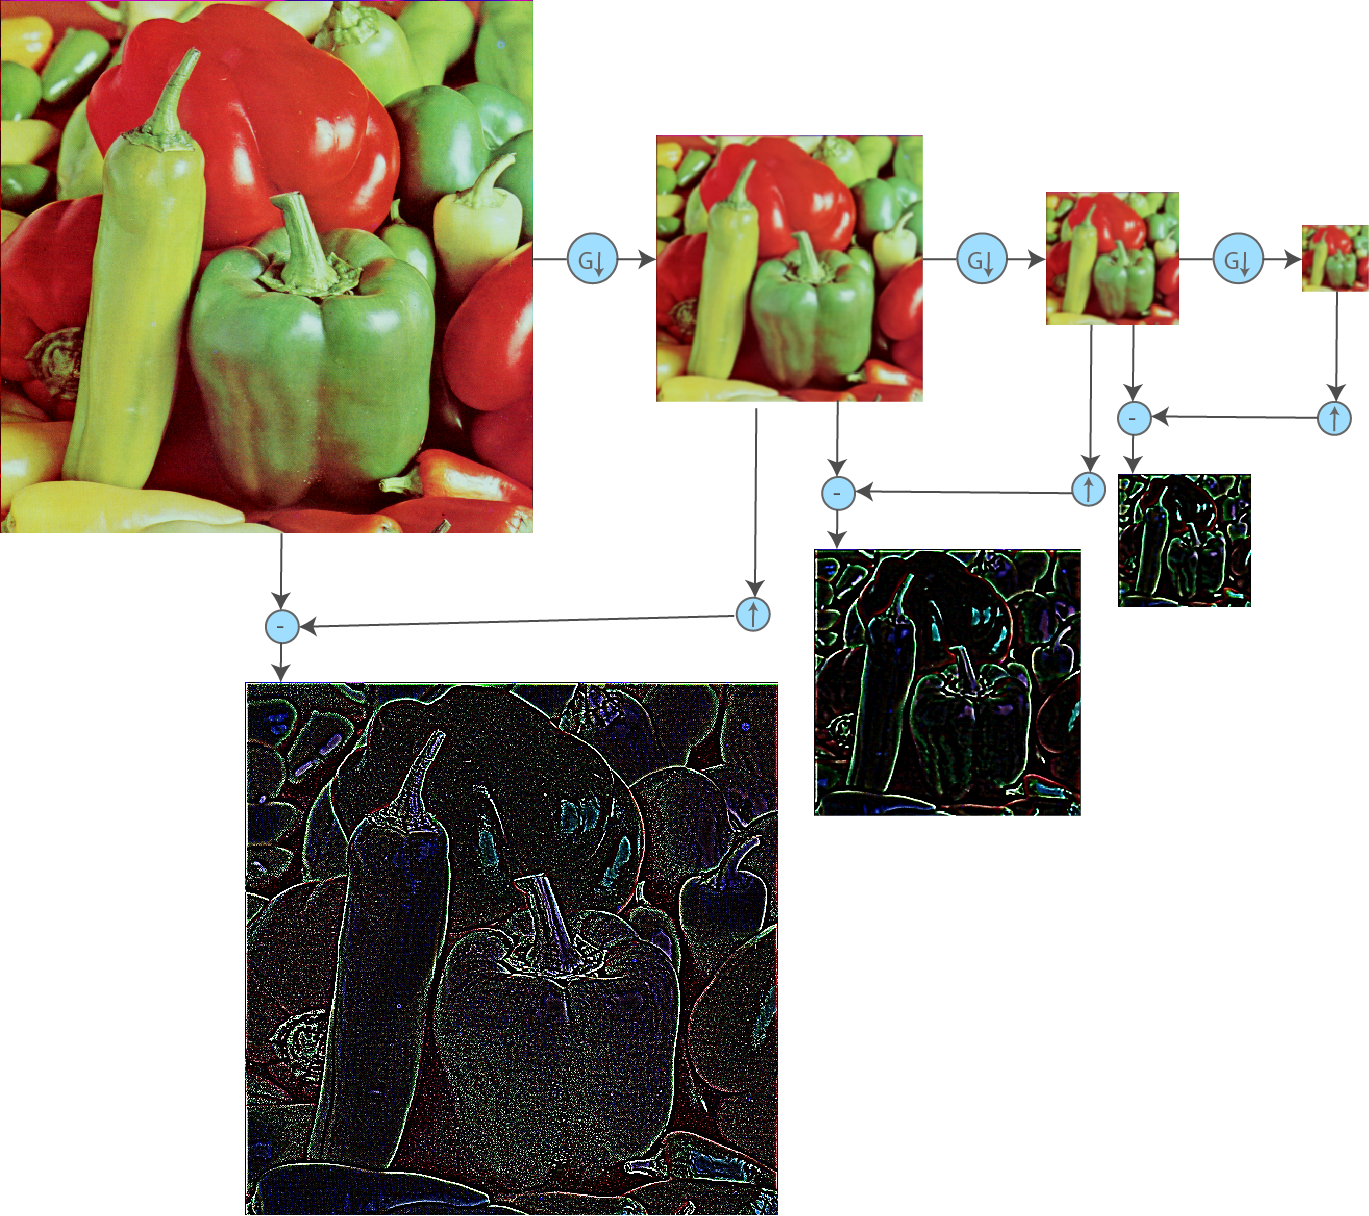
\includegraphics[width=\textwidth]{figures/peppers/laplacian_pyramid}
	\caption{Laplacian pyramid of an example image}
	\label{fig_pepper_laplacian_pyramid}
\end{figure}

The property of the Laplacian that makes it ideal for fusion is its ability to capture the high frequency components in an image through the use of very simple kernel operators that are easily implemented in hardware. The difference between a blurred image and the original will have higher magnitude in the areas where the image was sharpest.

The fusion of two images can be thought of as a function of the two images $X$ and $Y$ of dimension $M \times N$ where $Z = f(X, Y)$, a single image of dimension $M \times N$. A naive approach to fusion would be to compute the Laplacians and use their magnitudes to select a pixel from either $X$ or $Y$ as shown in Equation \ref{eq_naive_fusion}. In this context, $|L(x)|$ represents the absolute value of the Laplacian of the input.

\begin{equation}
Z(i,j)=
\begin{cases}
X(i,j) & |L(X(i,j))| \ge |L(Y(i,j))| \\
Y(i,j) & otherwise
\end{cases}
\label{eq_naive_fusion}
\end{equation}

This approach does not account for variations in colorspace between the two images. Consider the images in Figure \ref{fig_peppers_lr}. The more saturated image will likely have a higher valued Laplacian in some parts simply because it is brighter, therefore having higher magnitudes at individual pixels. This approach also will not facilitate smooth stitching of the images. Contiguous regions of selection from one image will be adjacent to regions from the other with no transition, producing a grainy effect at areas of high frequency. The result of this naive fusion can be seen in Figure \ref{fig_naive_fusion} which exhibits the flaws of this approach.

\begin{figure}[h]
	\centering
	\begin{subfigure}[b]{0.45\textwidth}
		\centering
		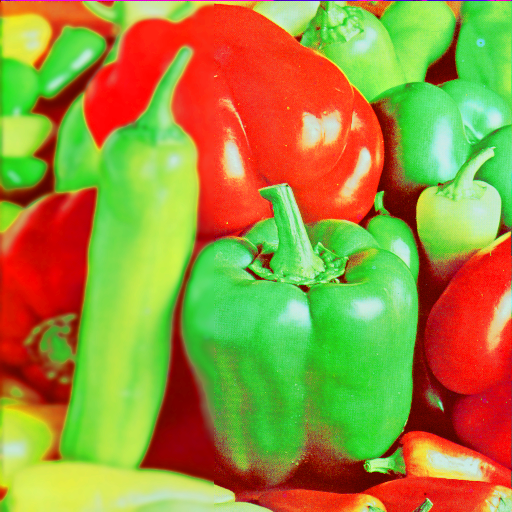
\includegraphics[width=\textwidth]{figures/peppers/peppers_blur_left}
		\caption{Blurred on the left; more saturated}
	\end{subfigure}
	\begin{subfigure}[b]{0.45\textwidth}
		\centering
		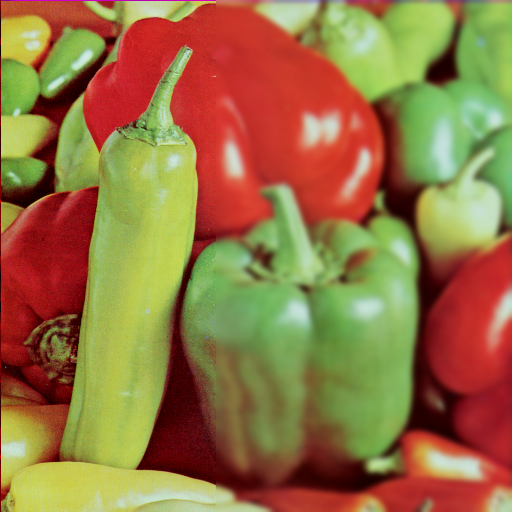
\includegraphics[width=\textwidth]{figures/peppers/peppers_blur_right}
		\caption{Blurred on the right; more neutral}
	\end{subfigure}
	\caption{Two images of the same scene with variations in sharpness and colorspace}
	\label{fig_peppers_lr}
\end{figure}

\begin{figure}[h]
	\centering
	\begin{subfigure}[b]{0.45\textwidth}
		\centering
		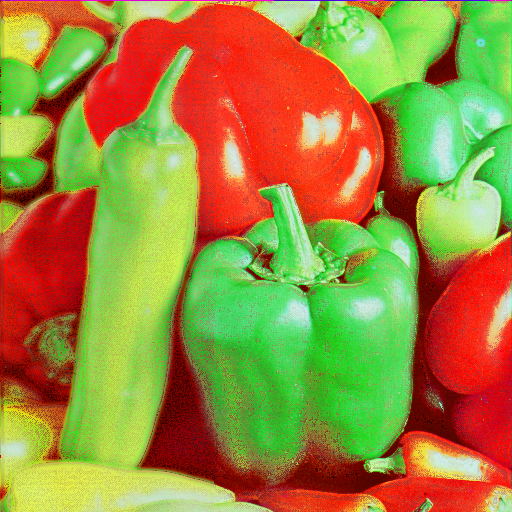
\includegraphics[width=\textwidth]{figures/peppers/peppers_fused_naive}
		\caption{Fusion using the naive approach}
		\label{fig_naive_fusion}
	\end{subfigure}
	\begin{subfigure}[b]{0.45\textwidth}
		\centering
		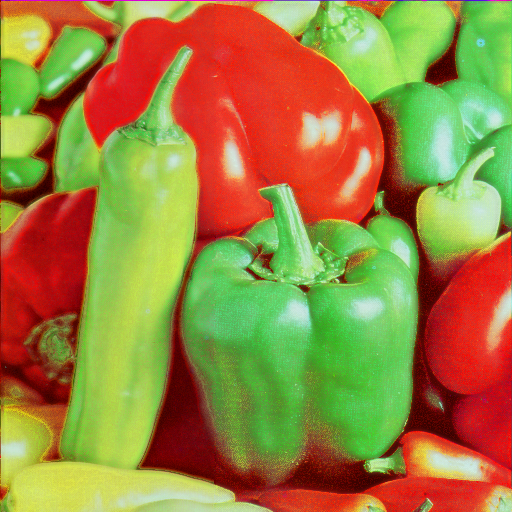
\includegraphics[width=\textwidth]{figures/peppers/peppers_fused}
		\caption{Fusion using weighted sum}
		\label{fig_weighted_fusion}
	\end{subfigure}
	\caption{Fusion of the images in Figure \ref{fig_peppers_lr} using a naive selection and weighted sum approach}
\end{figure}

A more correct approach would involve using the Laplacian in a weighted sum to combine the pixels of the images, rather than simply selecting them, as shown in Equation \ref{eq_weighted_fusion}.

\begin{equation}
Z(i,j) = \frac{|L(X(i,j))|}{|L(X(i,j))| + |L(Y(i,j))|} \cdot X(i,j) + \frac{|L(Y(i,j))|}{|L(X(i,j))| + |L(Y(i,j))|} \cdot Y(i,j)
\label{eq_weighted_fusion}
\end{equation}

The result of this weighted sum approach can be seen in Figure \ref{fig_weighted_fusion} which exhibits a reduction in graininess from the naive approach.

\subsection{Speeded-up Robust Features (SURF)}

The generation of features for use as marker points in alignment utilizes the SURF algorithm from Bay et al \cite{bay_surf:_2006}. SURF is composed of two parts: a discrete approximation for computing Hessian determinants, and the generation of rotation invariant feature descriptors for detected feature points. 

SURF is typically used for its applications in object recognition, where the feature descriptor is used to facilitate a match between what is observed and some known set of feature points and descriptors. The descriptor largely serves as a way of discriminating against false positives. In terms of using SURF for fusion, the detected feature points will be matched across two images with the assumption that the subject is the same and that the images do contain spatially coherent matches. Given this assumption, it can be concluded that the feature descriptor is not necessary for alignment. The feature points computed using Hessian determinants are sufficient.

\subsubsection{Computation of Hessian Determinants}

The Hessian determinant is the determinant of a Hessian matrix, which is a matrix composed of the spatial partial second derivatives of a function $f : \mathbb{R}^n \rightarrow \mathbb{R}$. It is of the general form shown in Equation \ref{eq_hessian_general}. In the image domain, $f : \mathbb{R}^2 \rightarrow \mathbb{R}$. The particular form of the Hessian matrix in $\mathbb{R}^2$ with dimensions $x_1$ and $x_2$ is shown in Equation \ref{eq_hessian_r2}.

\begin{equation}
H = \begin{bmatrix}
\frac{\partial^2 f}{\partial x_1^2} & \frac{\partial^2 f}{\partial x_1 x_2} & \cdots & \frac{\partial^2 f}{\partial x_1 \partial x_n} \\
\frac{\partial^2 f}{\partial x_2 \partial x_1} & \frac{\partial^2 f}{\partial x_2^2} & \cdots & \frac{\partial^2 f}{\partial x_2 \partial x_2} \\
\vdots & \vdots & \ddots & \vdots \\
\frac{\partial^2 f}{\partial x_n \partial x_1} & \frac{\partial^2 f}{\partial x_n \partial x_2} & \cdots & \frac{\partial^2 f}{\partial x_n^2}
\end{bmatrix}
\label{eq_hessian_general}
\end{equation}

\begin{equation}
H = \begin{bmatrix}
\frac{\partial^2 f}{\partial x_1^2} & \frac{\partial^2 f}{\partial x_1 x_2} \\
\frac{\partial^2 f}{\partial x_2 x_1} & \frac{\partial^2 f}{\partial x_2^2}
\end{bmatrix}
\label{eq_hessian_r2}
\end{equation}

The second order derivative used can be computed via convolution of the Gaussian second order derivative at any point, $x$, in the image. The formulas for the Gaussian second order derivative for each partial with respect to $x_1^2$, $x_1 x_2$ and $x_2^2$ can be seen in Equations \ref{eq_partial_x1}, \ref{eq_partial_x1x2}, and \ref{eq_partial_x2} respectively.

\begin{equation}
\frac{\partial^2 G(x_1,x_2,\sigma)}{\partial x_1^2} = (-1 + \frac{x_1^2}{\sigma^2})\frac{e^{-\frac{x_1^2+x_2^2}{2\sigma^2}}}{2\pi \sigma^4}
\label{eq_partial_x1}
\end{equation}

\begin{equation}
\frac{\partial^2 G(x_1,x_2,\sigma)}{\partial x_1 x_2} = \frac{x_1 x_2}{2 \pi \sigma^6}e^{-\frac{x_1^2 + x_2^2}{2 \sigma^2}}
\label{eq_partial_x1x2}
\end{equation}

\begin{equation}
\frac{\partial^2 G(x_1,x_2,\sigma)}{\partial x_2^2} = (-1 + \frac{x_2^2}{\sigma^2})\frac{e^{-\frac{x_1^2+x_2^2}{2\sigma^2}}}{2\pi \sigma^4}
\label{eq_partial_x2}
\end{equation}

3D surface plots of these equations where $\sigma=1$ can be seen in Figure \ref{fig_gaussian_surface_plots}. In order to compute these functions quickly, SURF approximates them with cropped, discrete, kernels. 

\begin{figure}[h]
	\centering
	\begin{subfigure}[b]{0.45\textwidth}
		\centering
		\includegraphics[width=\textwidth]{figures/hessian/gaussian_xx}
		\caption{$\frac{\partial^2 G(x_1, x_2)}{\partial x_1^2}$}
	\end{subfigure}
	\begin{subfigure}[b]{0.45\textwidth}
		\centering
		\includegraphics[width=\textwidth]{figures/hessian/gaussian_xy}
		\caption{$\frac{\partial^2 G(x_1, x_2)}{\partial x_1 x_2}$}
	\end{subfigure}
	\begin{subfigure}[b]{0.45\textwidth}
		\centering
		\includegraphics[width=\textwidth]{figures/hessian/gaussian_yy}
		\caption{$\frac{\partial^2 G(x_1, x_2)}{\partial x_2^2}$}
	\end{subfigure}
	\caption{3D surface plots of the Gaussian second order derivative functions where $\sigma=1$}
	\label{fig_gaussian_surface_plots}
\end{figure}

The Gaussian second order derivatives can be approximated as $9 \times 9$ kernels with $\sigma=1.2$. These kernels can be seen in Figure \ref{fig_gaussian_kernels}. By adjusting $\sigma$, Hessian determinants can be computed in different scale spaces. This is a concept that SURF draws from the Scale-Invariant Feature Transform (SIFT) from Lowe et al \cite{lowe_distinctive_2004}.

 By detecting features in different scale spaces, SIFT and by proxy, SURF are robust to changes in scale. SIFT accomplished this by downsampling the image to detect at lower order scale spaces. SURF improved on this approach for speed by instead scaling the kernel.

\begin{figure}[h]
	\centering
	\begin{subfigure}[b]{0.3\textwidth}
		\centering
		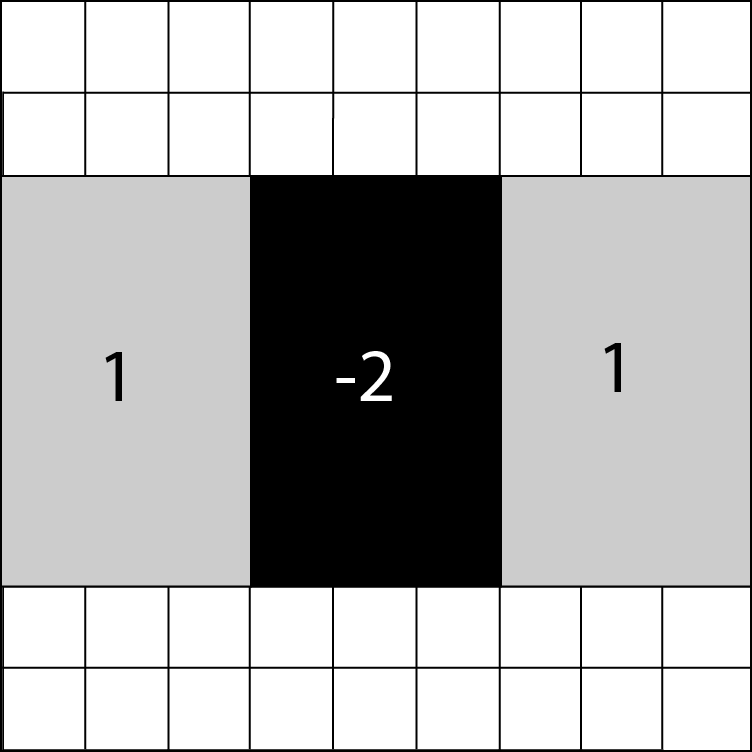
\includegraphics[width=\textwidth]{figures/hessian/gaussian_second_order_kernel_xx}
		\caption{$\frac{\partial^2 G}{\partial x_1^2}$}
	\end{subfigure}
	\begin{subfigure}[b]{0.3\textwidth}
		\centering
		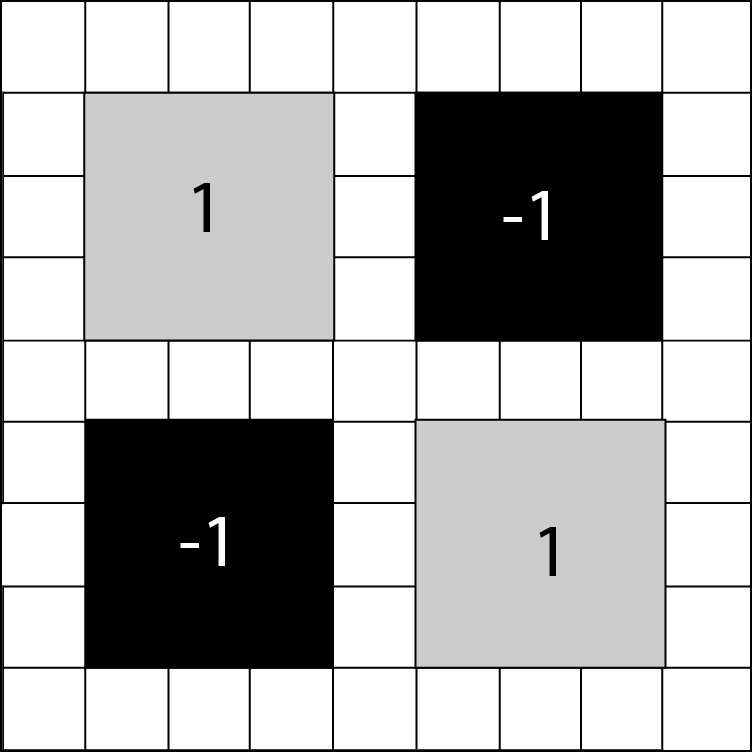
\includegraphics[width=\textwidth]{figures/hessian/gaussian_second_order_kernel_xy}
		\caption{$\frac{\partial^2 G}{\partial x_1 x_2}$}
	\end{subfigure}
	\begin{subfigure}[b]{0.3\textwidth}
		\centering
		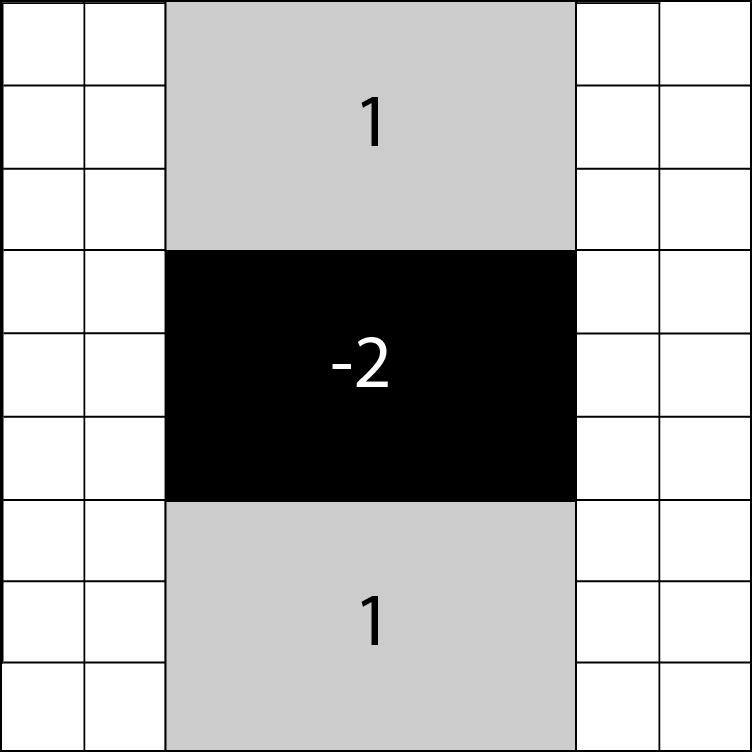
\includegraphics[width=\textwidth]{figures/hessian/gaussian_second_order_kernel_yy}
		\caption{$\frac{\partial^2 G}{\partial x_2^2}$}
	\end{subfigure}
	\caption{$9 \times 9$ discrete approximations of the Gaussian second order derivative with $\sigma=1.2$}
	\label{fig_gaussian_kernels}
\end{figure}

Another speed optimization presented in SURF takes advantage of the form of the discrete kernels. Since the approximated kernels are composed of rectangles of constant value, they can be decomposed into a set of box filters. Box filters can be computed quickly with the use of integral images. The general form of the integral image of an $M \times N$ image $I$ is shown in Equation \ref{eq_integral_image}.

\begin{equation}
\int I = \begin{bmatrix}
I(0,0) & \sum\limits_{m=0}^1 I(0,m) & \cdots & \sum\limits_{m=0}^M I(0,m) \\
\sum\limits_{n=0}^1 I(n,0) & \sum\limits_{n=0}^1 \sum\limits_{m=0}^1 I(n,m) & & \vdots \\
\vdots & & \ddots & \vdots \\
\sum\limits_{n=0}^N I(n,0) & \cdots & \cdots & \sum\limits_{n=0}^N \sum\limits_{m=0}^M I(n,m)
\end{bmatrix}
\label{eq_integral_image}
\end{equation}

Integral images decrease the computational complexity of finding the sum of an area in the input image. The computational complexity of strict kernel convolution at a point scales with the size of the kernel and is of the order $O(N^2)$ where the kernel is $N \times N$. A box filter can be decomposed into finding the sum of an area in the image and scaling it. Finding the sum from the integral image can be performed in $O(1)$ as shown in Equation \ref{eq_integral_image_box}. 

\begin{equation}
\sum\limits_{n=w}^y \sum\limits_{m=x}^z = \int I(y,z) - \int I(w-1,z) - \int I(y,x-1) + \int I(w-1, x-1)
\label{eq_integral_image_box}
\end{equation}

This makes the computation of the Hessian matrix scale only in terms of the image size, yielding no additional penalty for operating on different scale spaces.

\subsubsection{SURF Implementations for FPGA Devices}

The relatively low computational complexity makes SURF a popular choice for FPGA applications. Battezzati et al. present an architecture using accumulators for computing the integral image pipelined through the Hessian computation and storing detected feature points in a FIFO cache \cite{battezzati_surf_2012}. These are matched against a stored set of feature points. Chen et al. present improvements on this approach by parallelizing the computation of different scale spaces \cite{chen_fpga-based_2016}. The implementation in this thesis follows these approaches with some additional improvements for speed based on the use case of matching against another image rather than a stored set of features.

\subsection{Iterative Closest Point Algorithm}

The crucial step in aligning the two images is the computation of an affine transform mapping one image into the space of the other. Once the images are aligned, they can be fused. A combination of SURF and the iterative closest point algorithm are used to compute this transform. Iterative closest point was first proposed by Chen and Medioni as a method for aligning 3-D point cloud data \cite{chen_object_1992}. In its simplest form, the algorithm follows the following steps:

\begin{enumerate}
	\item Each point in the set of points to be transformed is matched against the closest (usually Euclidean distance) point in the reference set of points.
	\item A transformation is estimated to minimize the distance between the transform set and their matches in the reference set of points.
	\item The transform is applied to the points.
\end{enumerate}

This process is repeated, converging to the local minimum that is the match between the two point sets.

Let $X_p(i)$ be be the $i^{th}$ point in the set of reference points onto which the transform points, $X(j)$, where $j$ is the index of the closest point to $X_p(i)$ in $X$, will be projected. The general form for this transformation $M$ is shown in Equation \ref{eq_general_icp_mapping}, and the expanded matrix form can be seen in Equation \ref{eq_expanded_icp_mapping}. In the expanded matrix form $M$ is decomposed into $R$, a $2 \times 2$ rotation matrix, and $T$, a translation offset.

\begin{equation}
X_p(i) = X(j) \cdot M
\label{eq_general_icp_mapping}
\end{equation}

\begin{equation}
\begin{bmatrix}
X_p(i)_1 \\
X_p(i)_2 \\
1 
\end{bmatrix}
=
\begin{bmatrix}
X(j)_1 & X(j)_2 & 1
\end{bmatrix}
\cdot
\begin{bmatrix}
R_{11} & R_{12} & T_1 \\
R_{21} & R_{22} & T_2 \\
0 & 0 & 1
\end{bmatrix}
\label{eq_expanded_icp_mapping}
\end{equation}

This equation only solves for $M$ for a single point relation, but can be restructured to contain
the whole set of $N$ points as shown in Equation \ref{eq_full_icp_matrix}. In this equation $P$ is a function $P: i \rightarrow j$ mapping the closest points in each set.

\begin{equation}
\begin{bmatrix}
X_p(0)_1 \\
X_p(0)_2 \\
X_p(1)_1 \\
X_p(1)_2 \\
\vdots \\
X_p(N)_1 \\
X_p(N)_2
\end{bmatrix}
=
\begin{bmatrix}
X(P(0))_1 & X(P(0))_2 & 1 & 0 & 0 & 0 \\
0 & 0 & 0 & X(P(0))_1 & X(P(0))_2 & 1 \\
X(P(1))_1 & X(P(1))_2 & 1 & 0 & 0 & 0 \\
0 & 0 & 0 & X(P(1))_1 & X(P(1))_2 & 1 \\
\vdots & & & & & \vdots \\
X(P(N))_1 & X(P(N))_2 & 1 & 0 & 0 & 0 \\
0 & 0 & 0 & X(P(N))_1 & X(P(N))_2 & 1 
\end{bmatrix}
\cdot
\begin{bmatrix}
R_{11} \\
R_{12} \\
T_1 \\
R_{21} \\
R_{22} \\
T_2
\end{bmatrix}
\label{eq_full_icp_matrix}
\end{equation}

Solving for $M$ in this way maps all points in $X$ to their closest points in $X_p$ based on an orthogonal projection with the error minimized in a least-squares sense. 

In this form, the transform $M$ will include shear transformations and non-uniform scaling. The computation can be simplified by forcing the second basis vector in $R$ to be orthogonal to the first. The two cameras are expected to be be physically in the same plane, and as such, non-uniform scaling and shear transformations are not expected for alignment. By setting $R_{21} = -R_{12}$ and $R_{22} = R{11}$, the computation of $M$ can be reduced as shown in Equation \ref{eq_reduced_icp_matrix}.

\begin{equation}
\begin{bmatrix}
X_p(0)_1 \\
X_p(0)_2 \\
X_p(1)_1 \\
X_p(1)_2 \\
\vdots \\
X_p(N)_1 \\
X_p(N)_2
\end{bmatrix}
=
\begin{bmatrix}
X(P(0))_1 & X(P(0))_2 & 1 & 0 \\
X(P(0))_2 & -X(P(0))_1 & 0 & 1 \\
X(P(1))_1 & X(P(1))_2 & 1 & 0 \\
X(P(1))_2 & -X(P(1))_1 & 0 & 1 \\
\vdots & & & \vdots \\
X(P(N))_1 & X(P(N))_2 & 1 & 0 \\
X(P(N))_2 & -X(P(N))_1 & 0 & 1 \\
\end{bmatrix}
\cdot
\begin{bmatrix}
R_{11} \\
R_{12} \\
T_1 \\
T_2
\end{bmatrix}
\label{eq_reduced_icp_matrix}
\end{equation}

The performance of iterative closest point can be further improved by making it more sensitive to errors. Chetverikov introduces a variant of iterative closest point referred to as trimmed iterative closest point (TrICP) \cite{chetverikov_trimmed_2002}. TrICP is more robust to errors by eliminating points that introduce error into the matching. Some detected features points will not have correspondences between images. By eliminating these points, the overall error can be reduced to compute a more accurate transform.

\subsection{Singular Value Decomposition (SVD)}

Let Equation \ref{eq_reduced_icp_matrix} be of the form $X=Q \cdot M$. In order to compute the transform $M$, the equation must be restructured as in Equation \ref{eq_svd_inverse}.

\begin{equation}
Q^{-1} X = M
\label{eq_svd_inverse}
\end{equation}

$Q$ is not a square matrix, and as such is not invertible, but its pseudoinverse can be used in this instance. The pseudoinverse is computed through the use of singular value decomposition. The use of singular value decomposition to compute the transform is the source of the least squares fitting achieved by iterative closest point.

\subsubsection{SVD Implementations for FPGA Devices}

Ledesma-Carillo et al. present a hardware efficient algorithm for computing singular value decompositions on large matrices uisng one-sided Jacobi rotations \cite{ledesma-carrillo_reconfigurable_2011}.

\section{Implementation}

\subsection{Streaming Kernel Operators}

\subsubsection{Hessian Kernel with Accumulator}

\subsubsection{Box Kernel Approximation of Single Level Laplacian Pyramid}

\subsection{Computation of Transform from Detected Features}

\subsection{Application of Transform to Real-Time Data}

\section{Results}

\subsection{Selecting an optimal number of feature points}

A set of experiments to align the images shown in Figure \ref{fig_waterboy_left_right} were performed using different numbers of feature points for a variable number of iterations of the iterative closest point algorithm.

The iterative closest point algorithm always converges to a solution which minimizes the overall distance between the transform and reference set of points. This can be observed in Figure \ref{fig_results_error_plot} which shows the average distance from each point in the transform set of points to its closest neighbor in the reference set of points. Regardless of the selected number of features, all experiments converge to a roughly the same minimum. However, this may be an optimal solution in terms of distances between the feature points, but it is not always optimal in terms of alignment. 

\begin{figure}
	\centering
	\begin{subfigure}[b]{0.3\textwidth}
		\centering
		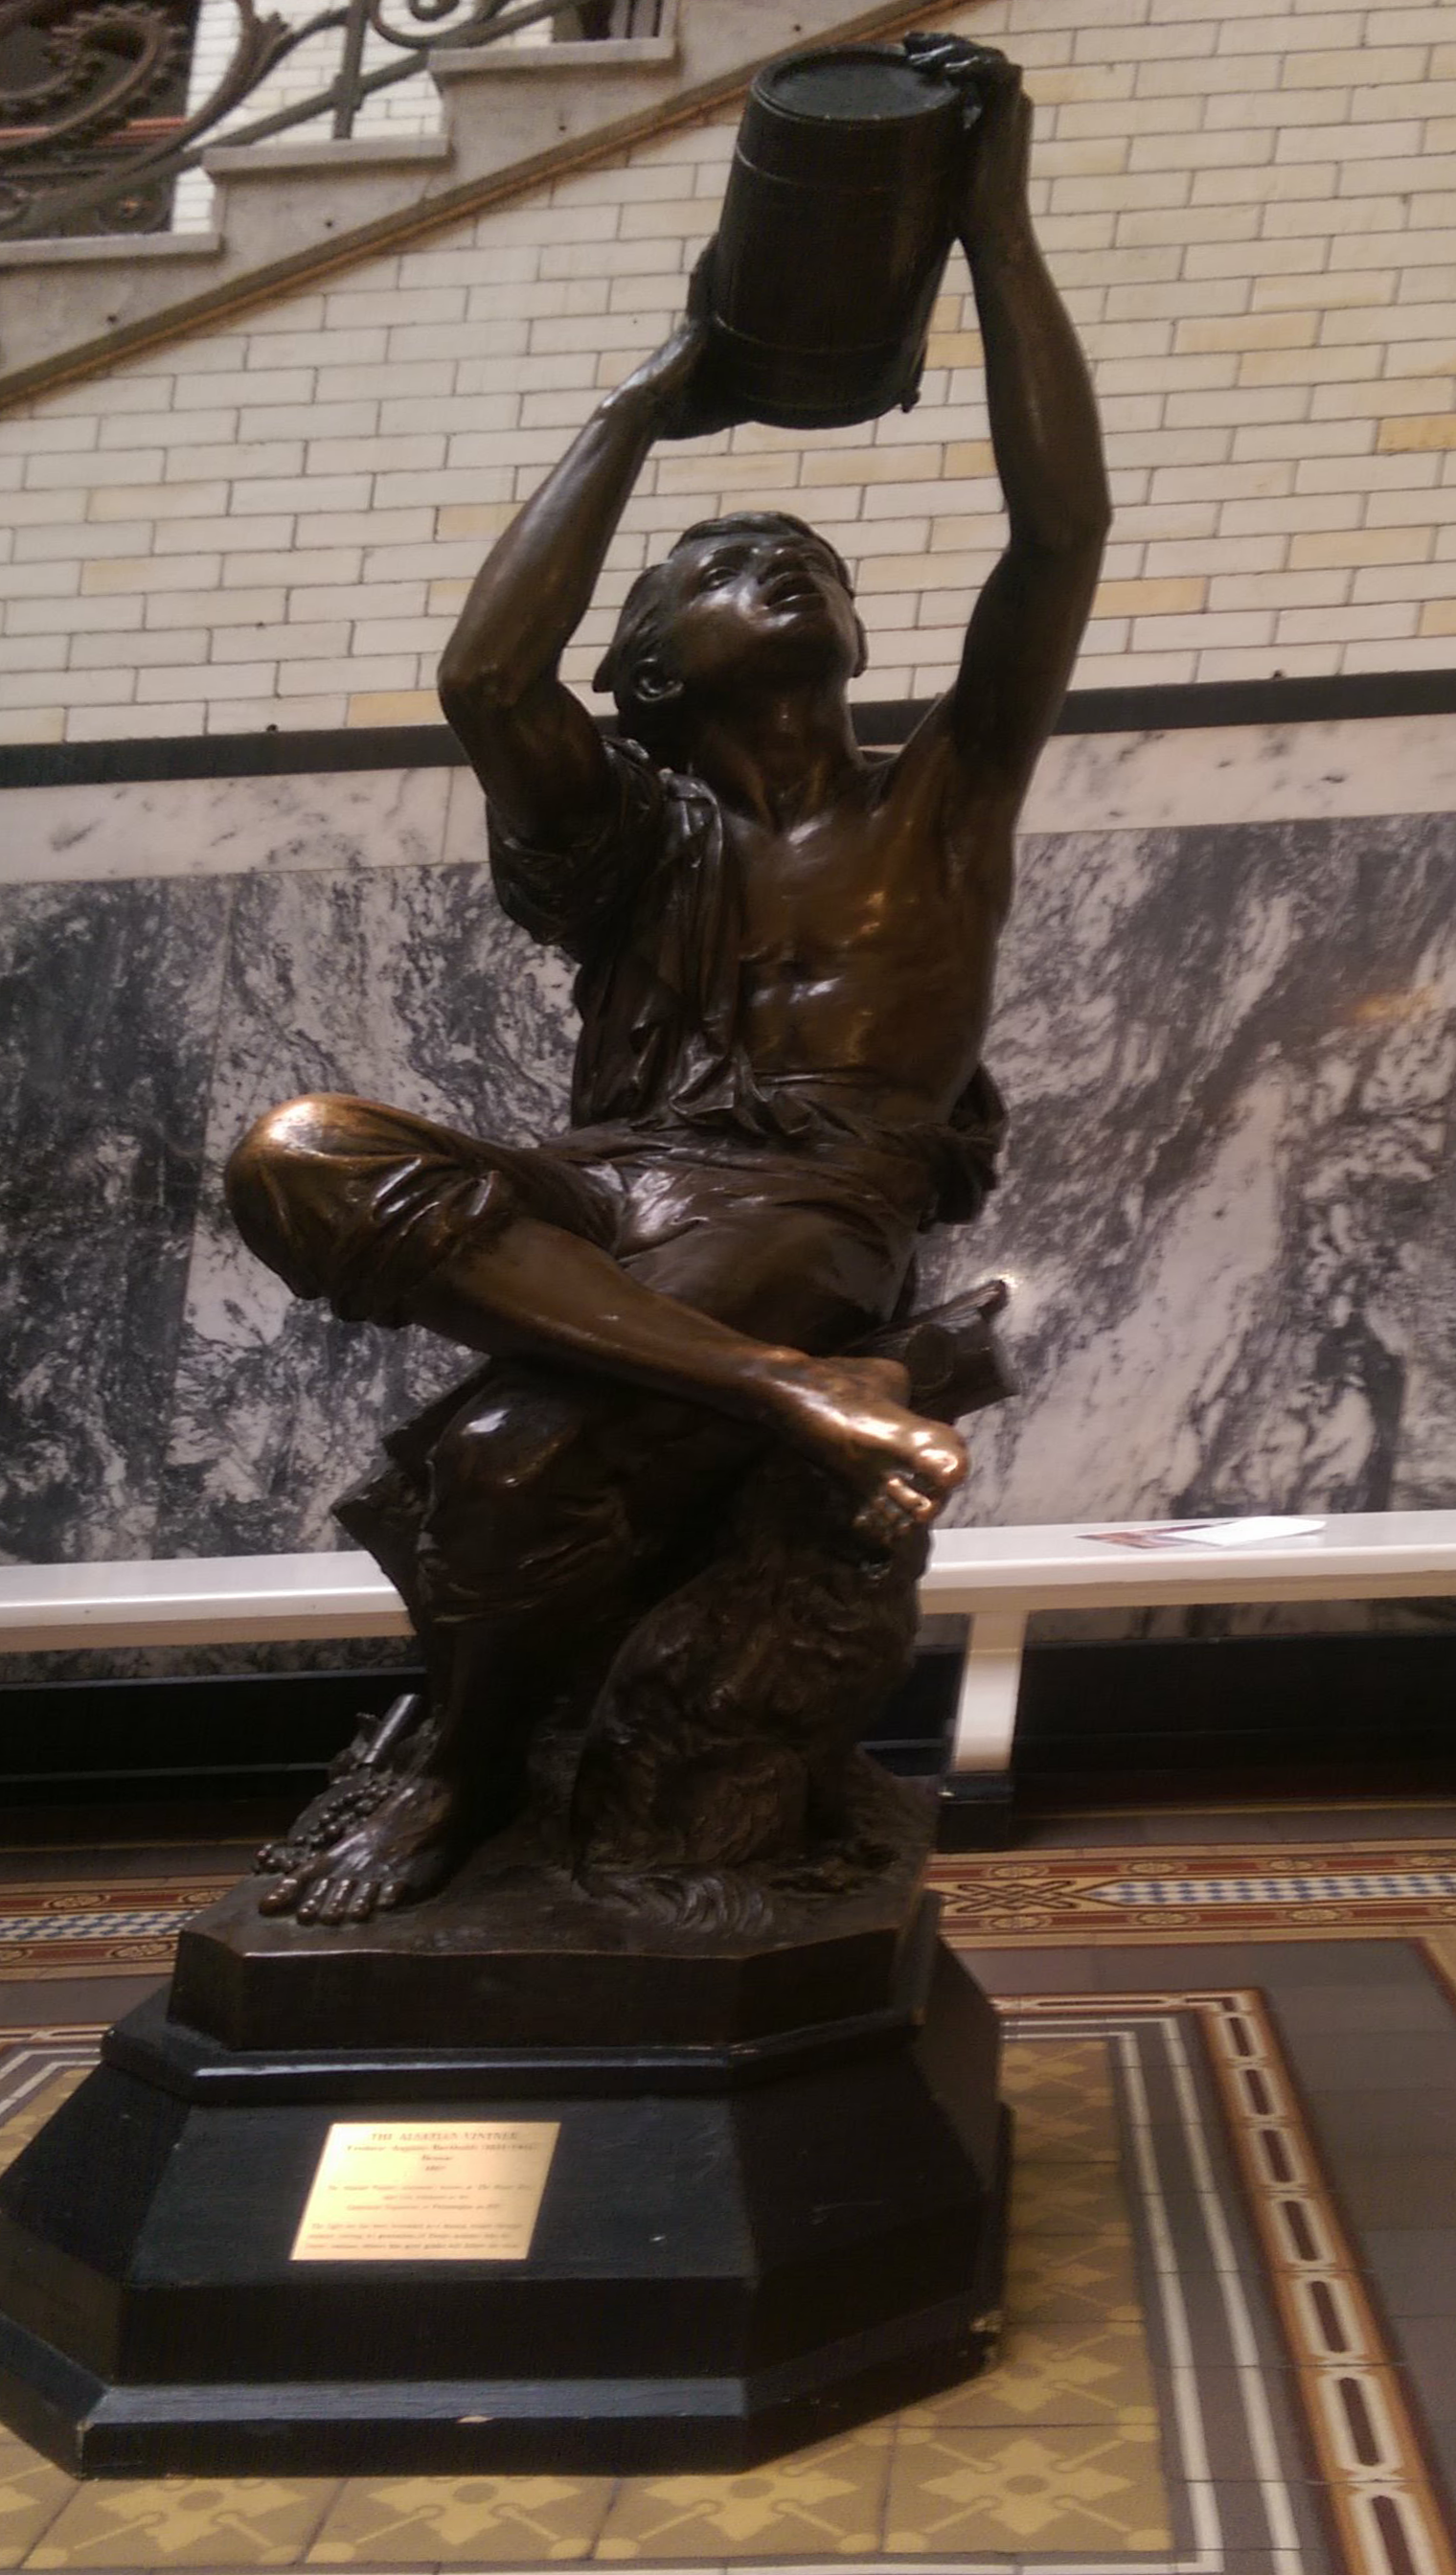
\includegraphics[width=\textwidth]{figures/alignment/waterboy_left}
		\caption{Reference Image}
	\end{subfigure}
	\begin{subfigure}[b]{0.3\textwidth}
		\centering
		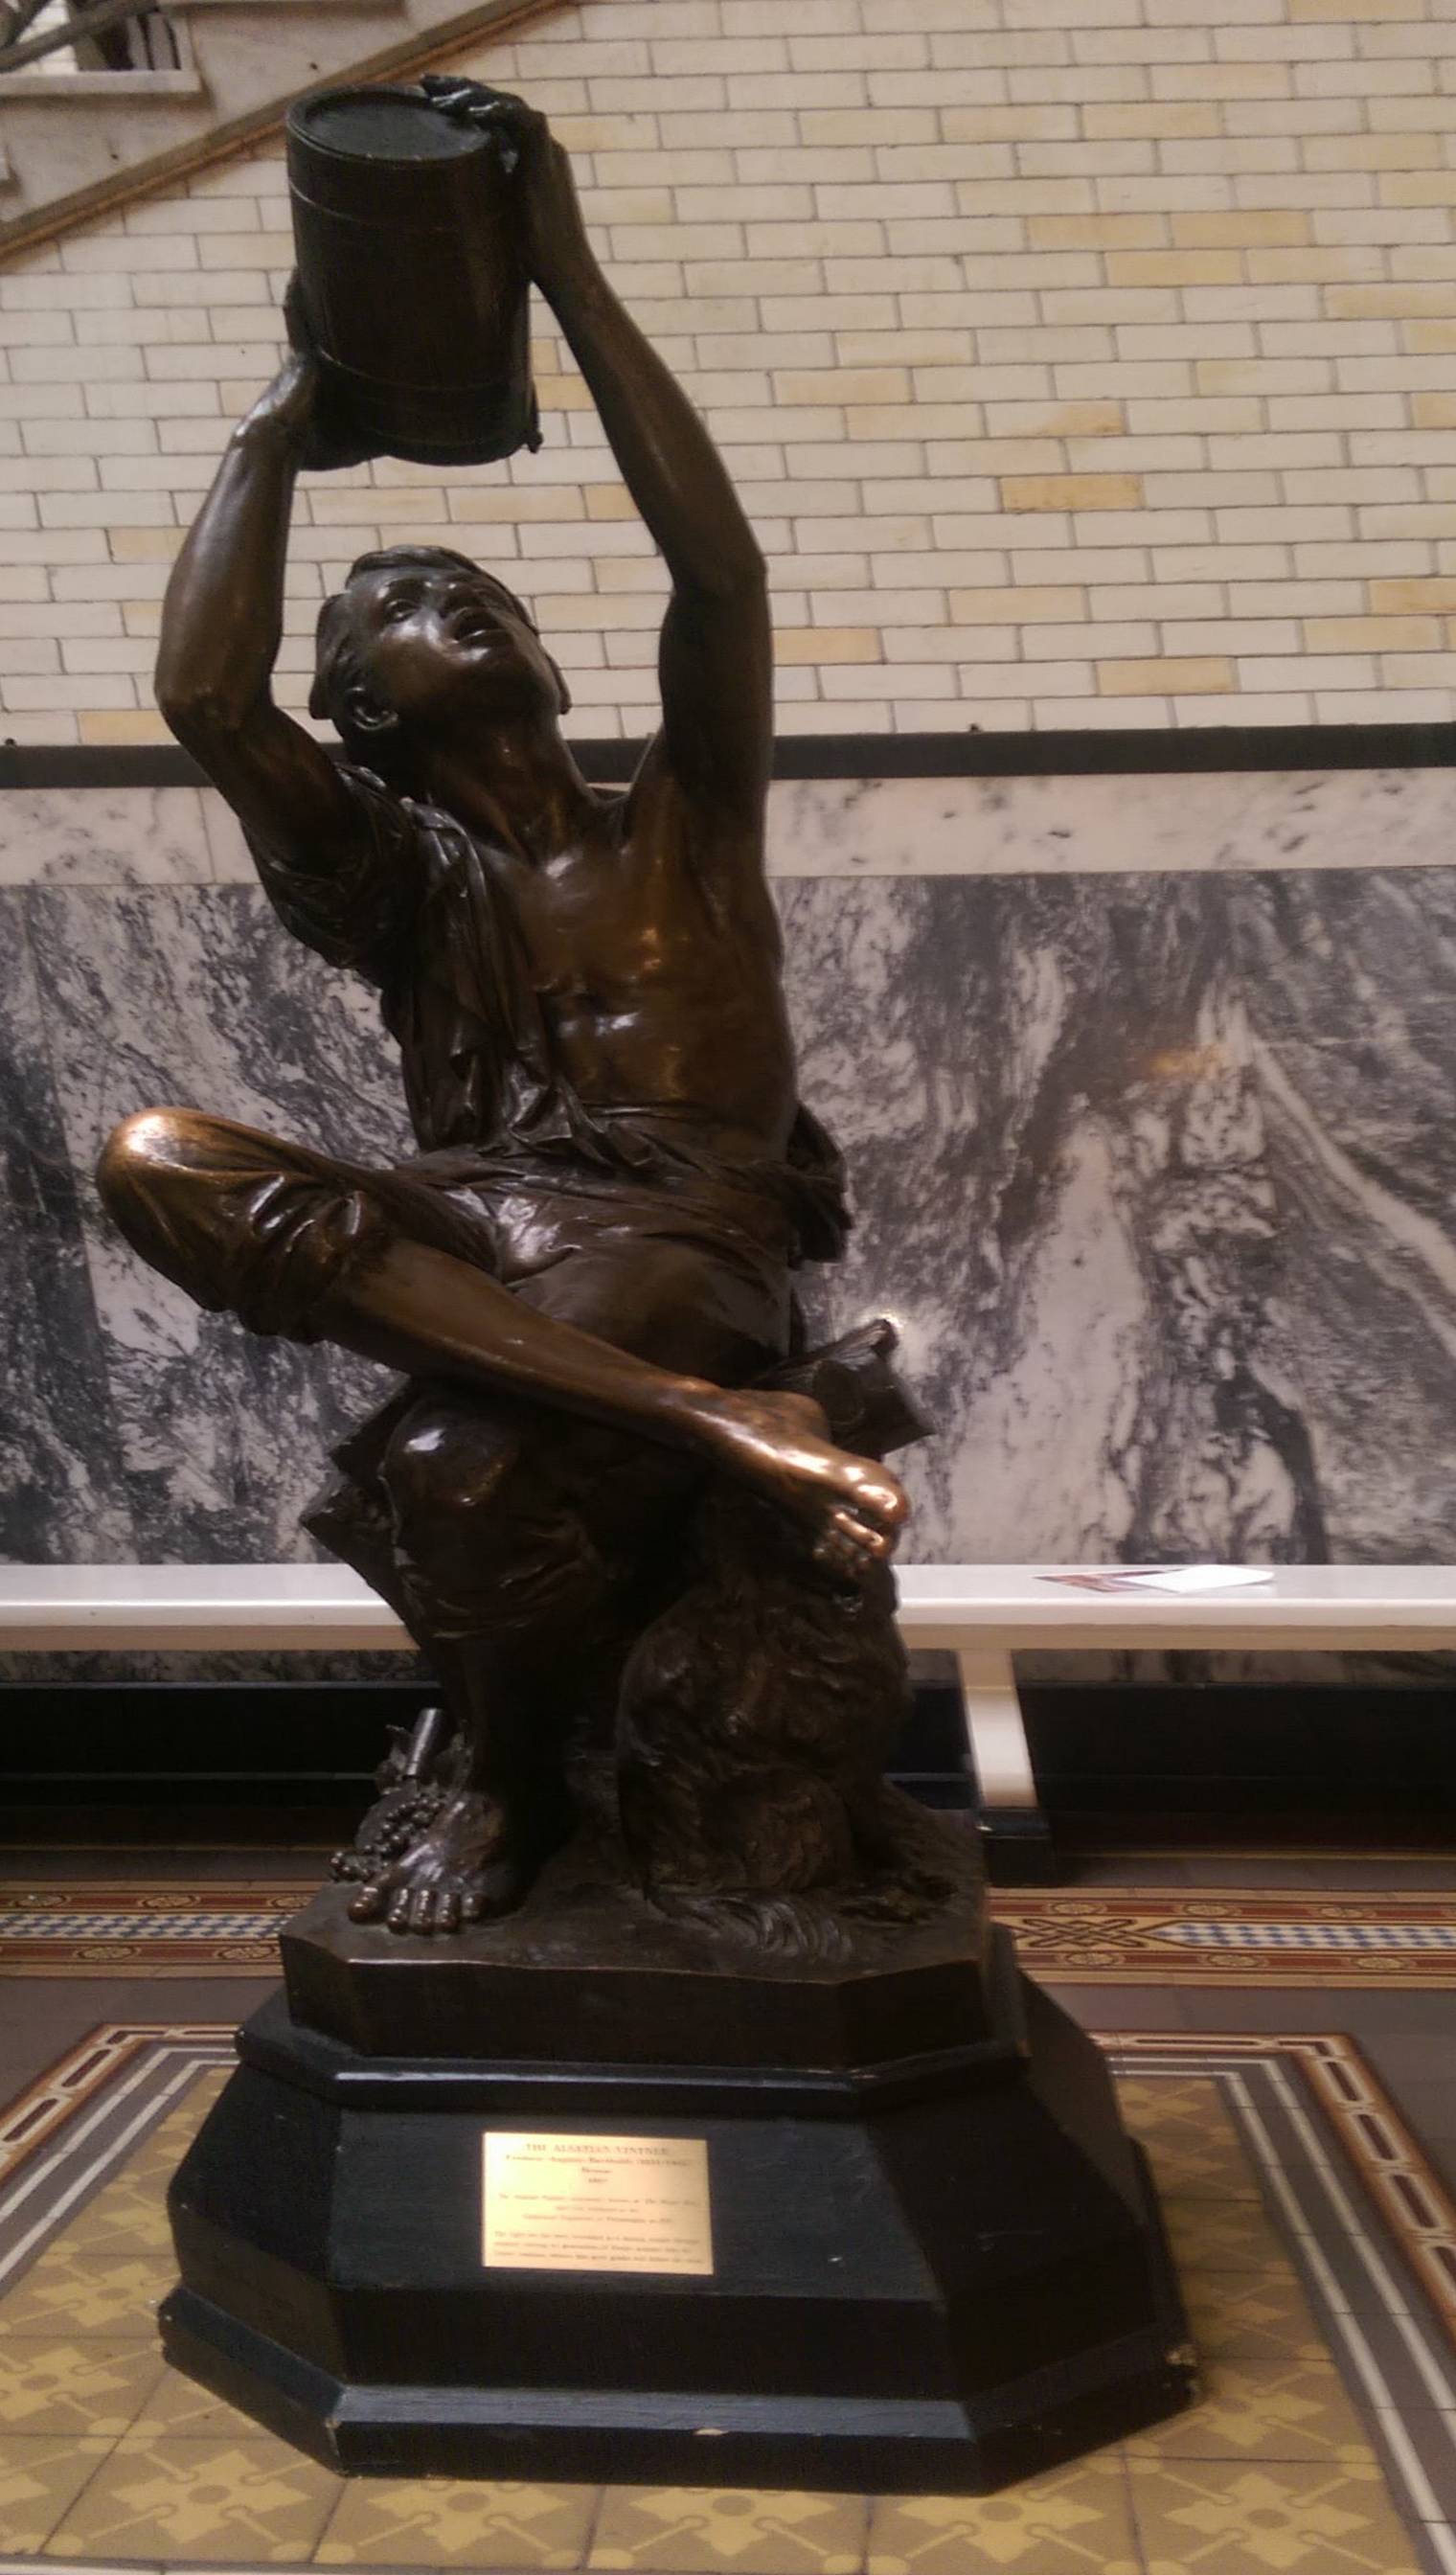
\includegraphics[width=\textwidth]{figures/alignment/waterboy_right}
		\caption{Transform Image}
	\end{subfigure}
	\caption{Images of "The Water Boy" by Frédéric-August Bartholdi from the Drexel Collection}
	\label{fig_waterboy_left_right}
\end{figure}

\begin{figure}[h]
	\centering
	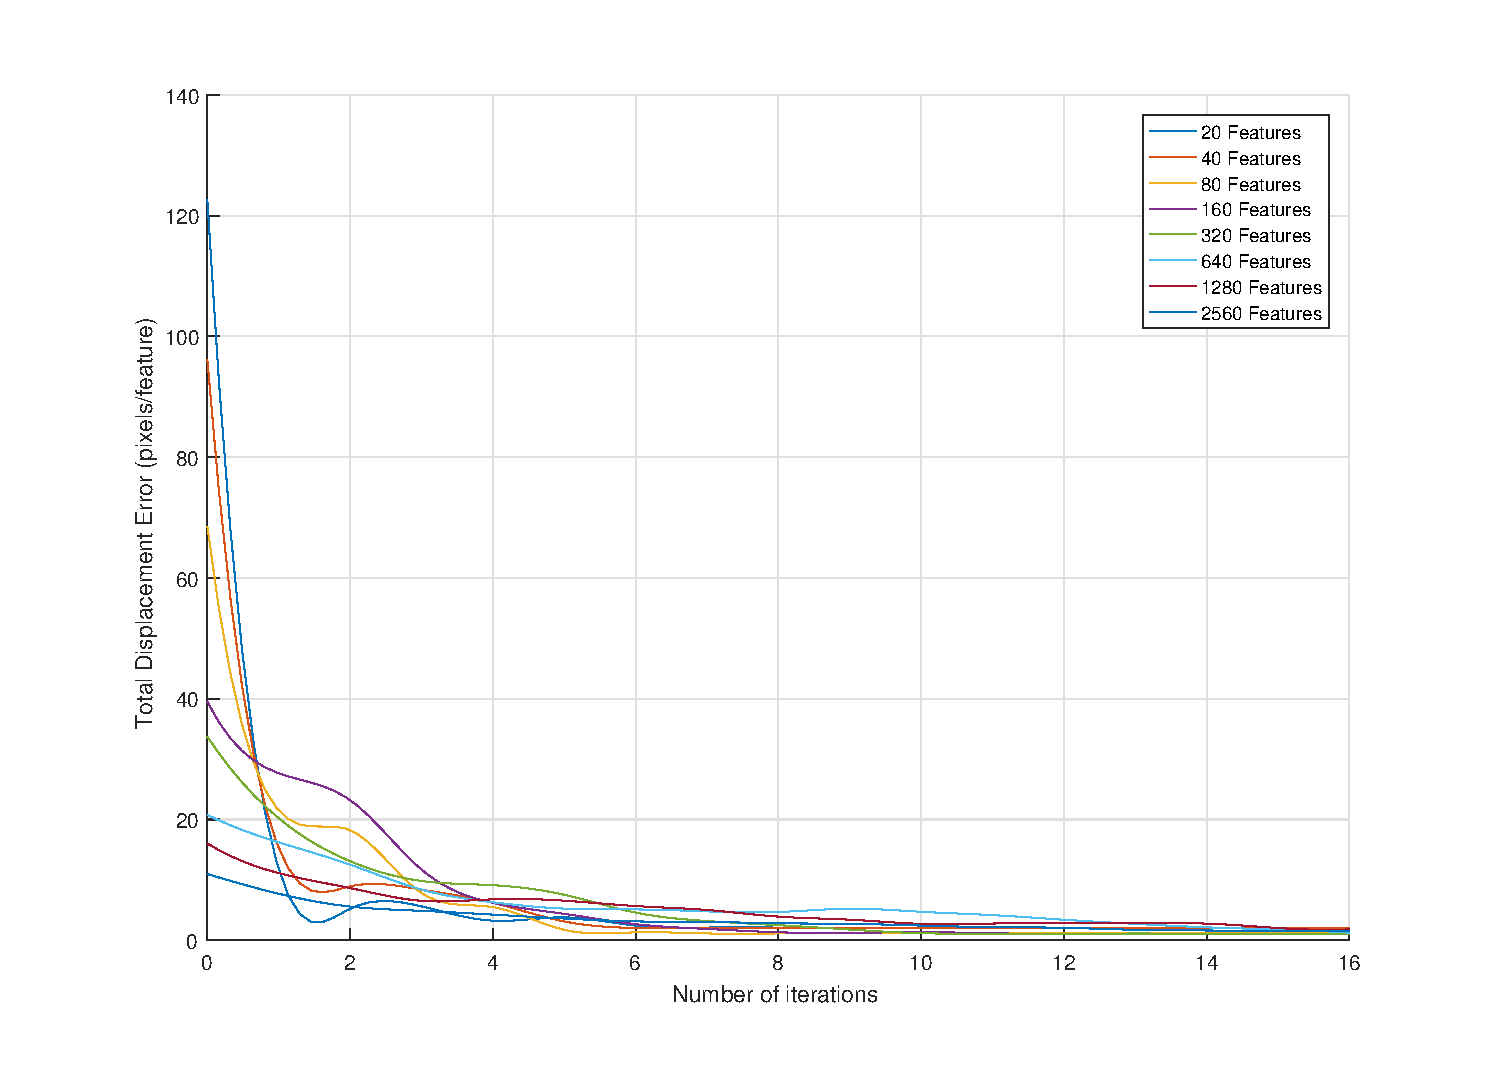
\includegraphics[width=\textwidth]{figures/alignment/error_for_iterations}
	\caption{The error in pixels per feature for performing $n$ iterations of the iterative closest point algorithm on differently sized sets of the strongest feature points}
	\label{fig_results_error_plot}
\end{figure}

Figure \ref{fig_alignment_results} shows the alignment between the transform and reference image when certain numbers of feature points are selected and used to compute the transform. It can be observed that $20$ features is not sufficient to compute a mapping, but that all of the images with more than $40$ features are imperfectly aligned. This is in spite of the fact that iterative closest point converges to a local minimum in terms of displacement error.

From this, it can be concluded that selecting a small, but sufficient number of feature points produces optimal alignment. This is likely due to the fact that additional feature points beyond just the strongest features in the images introduce error by trying to align the noisier parts of the background. A better error metric may be the one shown in Figure \ref{fig_results_alignment_error_plot} which shows the error in terms of the intensity difference. The magnitude of the overlaid image subtracted from the original is used to compute this error metric which more accurately reflects the alignment results shown in Figure \ref{fig_alignment_results}.

\begin{figure}[h]
	\centering
	\begin{subfigure}[b]{0.3\textwidth}
		\centering
		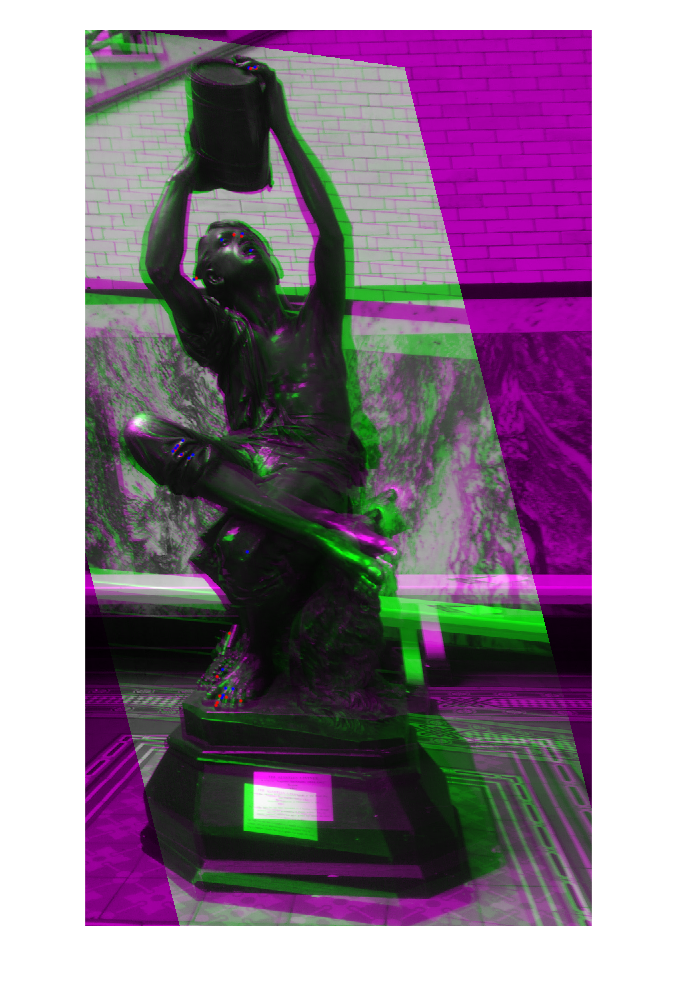
\includegraphics[width=\textwidth]{figures/alignment/fused_20_features_16_iterations}
		\caption{20 features}
	\end{subfigure}
	\begin{subfigure}[b]{0.3\textwidth}
		\centering
		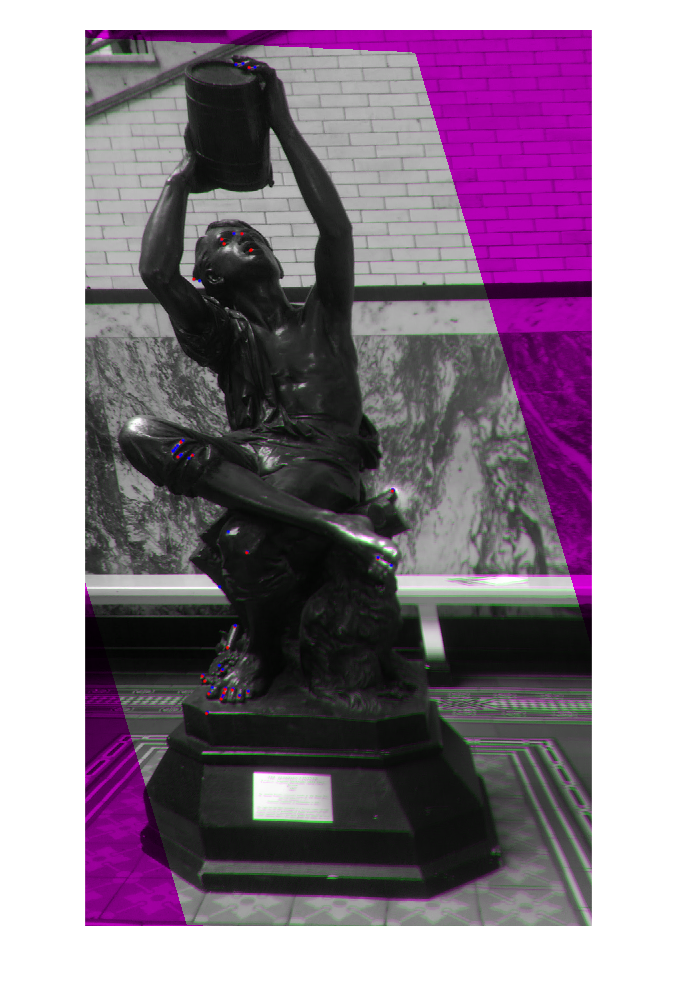
\includegraphics[width=\textwidth]{figures/alignment/fused_40_features_16_iterations}
		\caption{40 features}
	\end{subfigure}
	\begin{subfigure}[b]{0.3\textwidth}
		\centering
		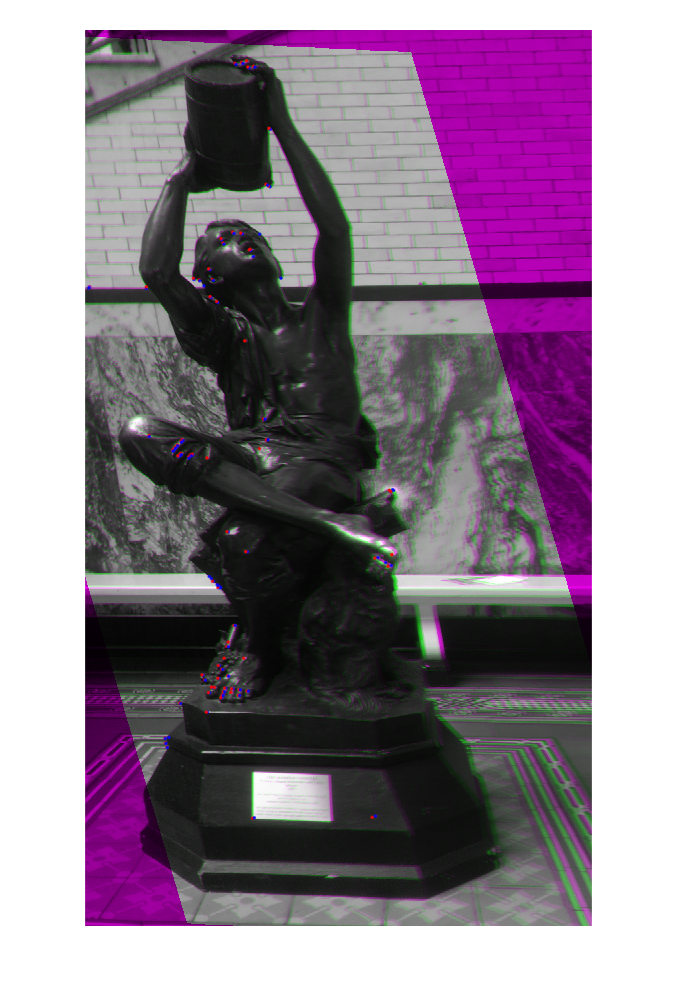
\includegraphics[width=\textwidth]{figures/alignment/fused_80_features_16_iterations}
		\caption{80 features}
	\end{subfigure}

   	\begin{subfigure}[b]{0.3\textwidth}
    	\centering
    	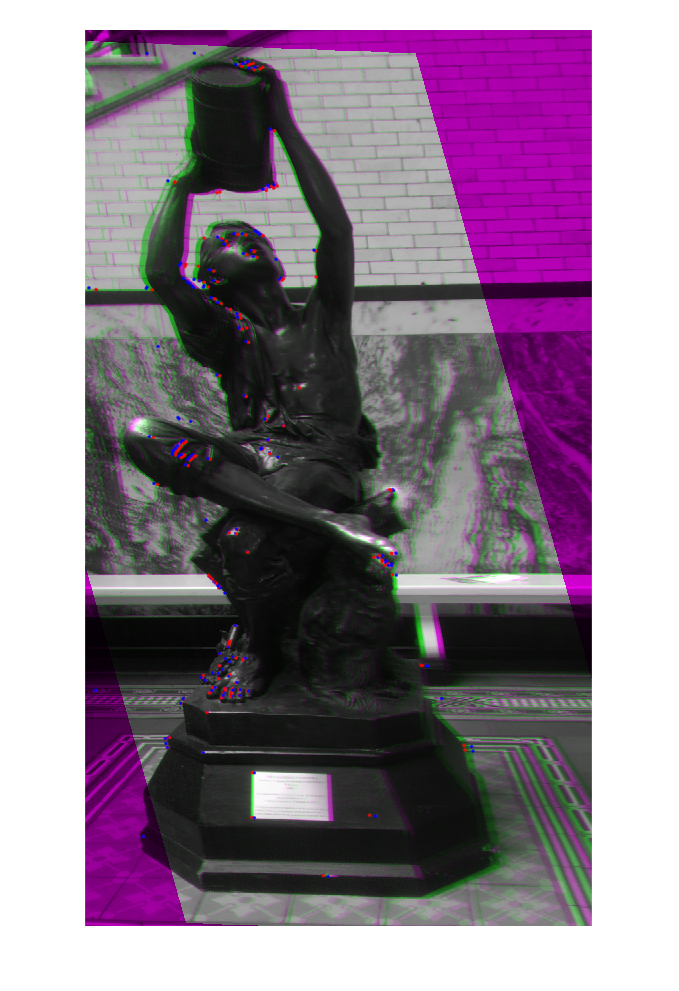
\includegraphics[width=\textwidth]{figures/alignment/fused_160_features_16_iterations}
    	\caption{160 features}
    \end{subfigure}
    \begin{subfigure}[b]{0.3\textwidth}
    	\centering
    	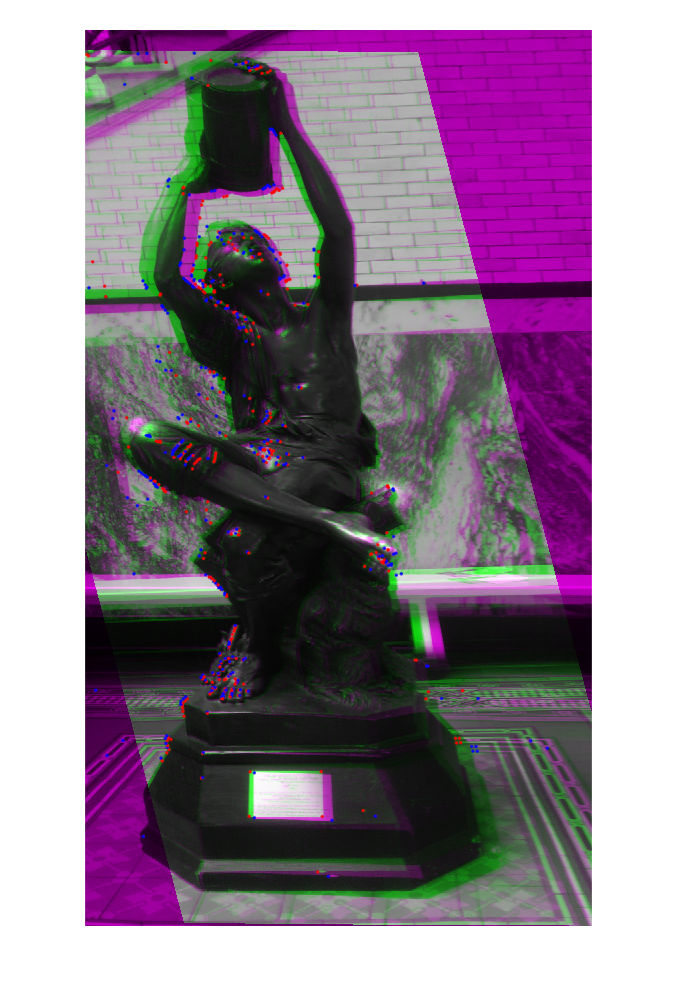
\includegraphics[width=\textwidth]{figures/alignment/fused_320_features_16_iterations}
    	\caption{320 features}
    \end{subfigure}
    \begin{subfigure}[b]{0.3\textwidth}
    	\centering
    	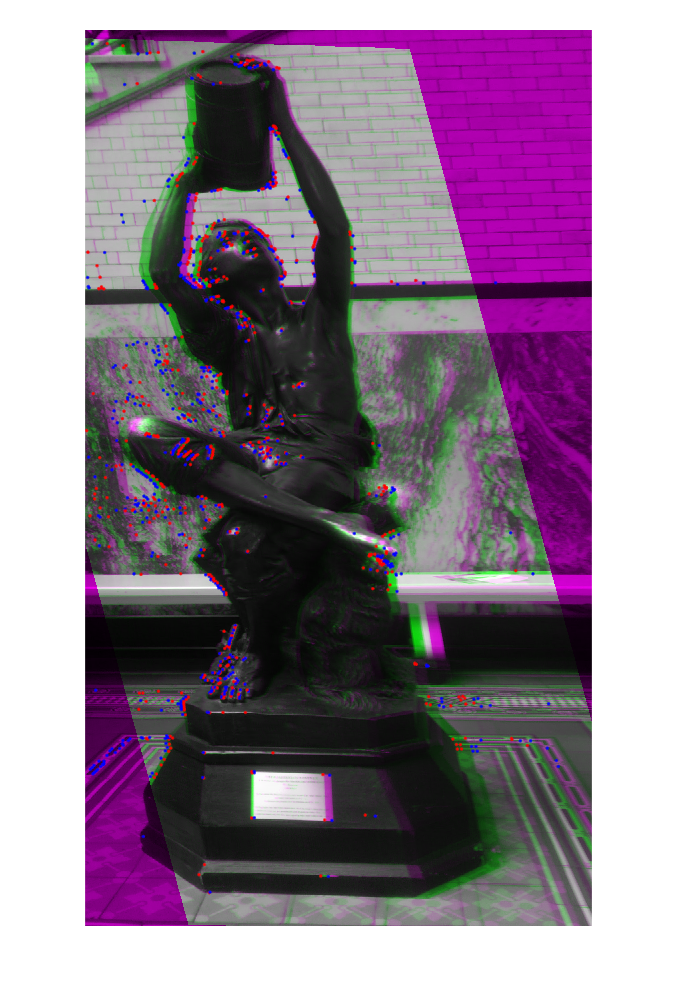
\includegraphics[width=\textwidth]{figures/alignment/fused_640_features_16_iterations}
    	\caption{640 features}
    \end{subfigure}
	\caption{Alignment results after running iterative closest point for 16 iterations on varying numbers of features with reference features marked in red and transformed features in blue}
	\label{fig_alignment_results}
\end{figure}

\begin{figure}[h]
	\centering
	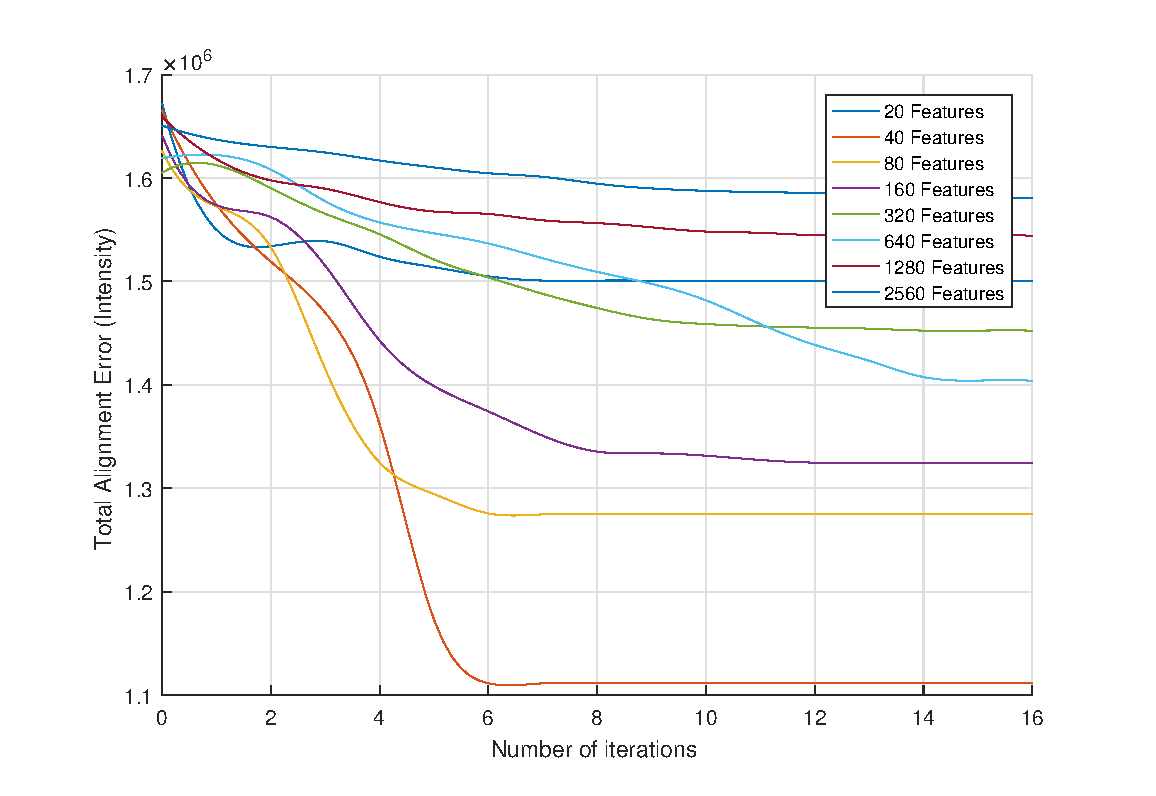
\includegraphics[width=\textwidth]{figures/alignment/error_for_alignment}
	\caption{The error in intensity based on the alignment from performing $n$ iterations of the iterative closest point algorithm on differently sized sets of the strongest feature points}
	\label{fig_results_alignment_error_plot}
\end{figure}

\pagebreak
\clearpage

\bibliographystyle{plain}
\bibliography{thesis}

\end{document}
